\section{Desenvolvimento do Problema}\label{sec:des_prob}
\AtBeginSec

\begin{frame}{Modelo de Sistema}
   \begin{bigitem}
      \item Considera-se um ambiente multi-canal OFDM com dois saltos, consistindo de uma ERB, uma ER (estação repetidora) fixa e uma EA (estação assinante)
      \item A estratégia de cooperação utilizada é DF.      
      \item É considerado AWGN, com variância $\sigma^2$ percebida por todas as subportadoras em todos os enlaces. 
      \item A eficiência espectral de cada subportadora, e.g. , no enlace ERB-ER é dada por
        \begin{equation}\label{eq:eff_spect}
           R_i^{s}(P_i^{s}) = \frac{1}{2N}\log_2\Big(1 + P_i^{s}g_i^{s}\Big).
        \end{equation}
   \end{bigitem}
\end{frame}

\begin{frame}{Modelo de Sistema}
   \begin{figure}[!htb]
     \centering
     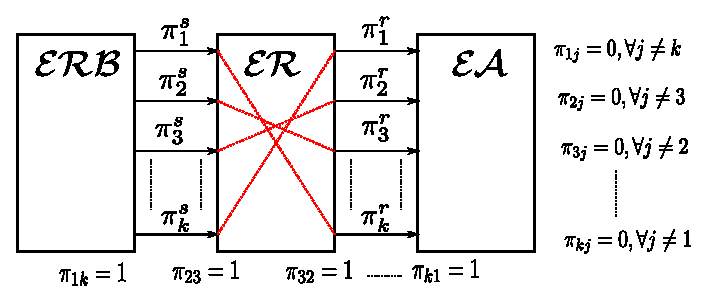
\includegraphics[width=0.7\linewidth]{../Imagens/schematic.eps}
     \caption{Esquemático de um ambiente OFDM com dois saltos.}\label{fig:schematic}
   \end{figure}
\end{frame}

\begin{frame}{Modelo de Sistema}
   \begin{bigitem}
      \item O prefixo cíclico OFDM e o tempo de coerência são considerados suficientemente longos e é assumido que todos os nós possuem sincronização de tempo e frequência perfeitos.
      \item Assume-se conhecimento total das informações do canal na ER.
      \item O desvanecimento em cada subportadora é independente.
      \item Consideramos comunicação entre as subportadoras de um para um.
   \end{bigitem}
\end{frame}

\begin{frame}{Formulação do Problema}
   \begin{bigitem}
      \item O problema de otimização conjunto do emparelhamento de subportadoras e alocação de potência pode ser escrito como
      \begin{subequations}\label{eq:conj_pro}
              \begin{alignat}{3}
                      \min_{P_i^s,P_i^r,\pi_{ij}}-\sum_{i=1}^N &\min\left\{R_i^s(P_i^s),\sum_{j=1}^N\pi_{ij}R_i^r(P_i^r)\right\},\\
                      \text{s.t.} &\sum_{i=1}^N P_i^s \leq P_{t}^s, \quad \sum_{j=1}^N P_i^r \leq P_{t}^r,\\
                      -&P_i^s \leq 0, \forall i, \quad -P_j^r \leq 0, \forall j,\label{seq:restP} \\
                      & \sum_{j}^N \pi_{j} = 1, \forall \quad 1 \leq j \leq N,\label{seq:restEmpr}\\
                      &\pi_{i,j} \in \{0, 1\}.
              \end{alignat}
      \end{subequations}
   \end{bigitem}
\end{frame}

%%%%%%%%%%%%%%%%%%%%%%%%%%%%%%% BACKUP  %%%%%%%%%%%%%%%%%%%%%%%

%\begin{frame}{Formulação do Problema}
%   \begin{bigitem}
%      \item O problema de otimização \eqref{eq:conj_pro} pode ser visto como um problema de otimização misto binário inteiro.
%      \item Ao separar o emparelhamento de subportadoras da alocação de potência, almejamos uma simplificação da solução para alocação de potência, para torná-lo um problema convexo.
%      \item O problema \eqref{eq:conj_pro} pode ser simplificado a partir de dois resultados que serão mostrados a seguir.
%   \end{bigitem}
%\end{frame}

% descomentar esse

%\begin{frame}{Emparelhamento Ótimo de Subportadoras para 2 saltos}
%   \begin{bigitem}
%      \item Assumimos que as subportadoras de ambos os saltos estão ordenadas em ordem decrescente em relação aos seus ganhos, i.e\ ,
%      \begin{equation}
%      g_1^s\geq g_2^s\geq \cdots \geq g_N^s \quad\text{e}\quad g_1^r\geq g_2^r\geq \cdots \geq g_N^r.
%      \end{equation}
%   \end{bigitem}
%   \begin{lemma}\label{lem:emparelhamento}
%     Existe uma solução ótima $(\boldsymbol{\pi}^*, P^{s*}, P^{r*})$ para \eqref{eq:conj_pro} tal que $\pi^*_{ii} = 1$, para todo $i=1,2,\ldots,N$.
%   \end{lemma}
%\end{frame}
%
%\begin{frame}{Emparelhamento Ótimo de Subportadoras para 2 saltos}
%   \begin{bigitem}
%      \item A ideia da demonstração da solução do Lema \ref{lem:emparelhamento} é construir uma solução ótima que seja igual à solução proposta, com o emparelhamento mostrado antes.
%      \item A demonstração é iterativa, chegando à solução ótima em no máximo N-1 passos.
%      \item Portanto, qualquer solução ótima para o emparelhamento de subportadoras terá no máximo eficiência igual ao esquema de emparelhamento proposto, que é de ordenar as subportadoras em ordem decrescente em relação aos ganhos.
%   \end{bigitem}
%\end{frame}

% retirar esses dois
%\begin{frame}{Alocação de Potência para o Emparelhamento Ótimo}
%   \begin{bigitem}
%      \item Ao eliminar o emparelhamento do problema \ref{eq:conj_pro}, chegamos a um problema de alocação de potência:
%      \begin{subequations}\label{eq:pot_emp_pro}
%              \begin{alignat}{3}
%                      \min_{P_i^s,P_i^r}-\sum_{i=1}^N &\min\left\{R_i^s(P_i^s),R_i^r(P_i^r)\right\},\\
%                      \text{s.t.} &\sum_{i=1}^N P_i^s \leq P_{t}^s,\\
%                      &\sum_{j=1}^N P_i^r \leq P_{t}^r,\\
%                      -&P_i^s \leq 0, \forall i, \quad -P_j^r \leq 0, \forall j\label{seq:match_restP}.
%              \end{alignat}
%      \end{subequations}
%   \end{bigitem}
%\end{frame}
%
%\begin{frame}{Alocação de Potência para o Emparelhamento Ótimo}
%   \begin{bigitem}
%      \item Para tratar o problema, utilizamos o Teorema \ref{teo:pot_lin_ret}
%   \end{bigitem}
%   \begin{theo}\label{teo:pot_lin_ret}
%   Existe uma solução ótima $(P^{s*},P^{r*})$ para \eqref{eq:pot_emp_pro} tal que a seguinte relação é mantida:
%     \begin{align}\label{eq:lin_rel_pot}
%        g_i^sP_i^s &= g_i^rP_i^r
%     \end{align}
%   \end{theo}
%\end{frame}
%
\begin{frame}{Alocação de Potência para o Emparelhamento Ótimo}
   \begin{bigitem}
      \item Após a solução do emparelhamento e utilizando essa relação, o problema pode ser reescrito como:
      \begin{subequations}\label{eq:q_pro}
        \begin{alignat}{3}
             (Q):\:\: \max         & \sum_{i=1}^{N} \ln \left( 1 + P^s_i \cdot g^s_i\right)  \label{seq:main_p}  \\
             \mbox{suj} :  & \sum_{i=1}^{N} P^s_i \leq P^s_t, \label{seq:restPsS}       \\
             & \sum_{i=1}^{N} \frac{g^s_i}{g^r_i}P^s_i \leq P^r_t,  \label{seq:restPrS}     \\
             & P^s_i \geq 0, \forall i. \label{seq:restNNS}
        \end{alignat}
      \end{subequations}
   \end{bigitem}
\end{frame}

\begin{frame}{Algoritmos Sub-ótimos}
   \begin{bigitem}
      \item A fim de simplificar a solução do problema \eqref{eq:q_pro}, foram propostos dois algoritmos sub-ótimos:
      \begin{bigitem}
         \item Water-Filling com Escalonamento de Potência.
         \item Water-Filling Mínimo.
      \end{bigitem}
      \item Quando as restrições \eqref{seq:restPsS} ou \eqref{seq:restPrS} não são consideradas, as relaxações propostas são as seguintes:
      \begin{align*}
      (Q^s): \; \max & \sum_{i=1}^{N} \ln \left( 1 + P^s_i g^s_i\right) & (Q^r): \; \max & \sum_{i=1}^{N} \ln \left( 1 + P^r_i  g^r_i\right) \\
      \text{suj :} \quad & \sum_{i=1}^{N} P^s_i \leq P^s_t,                 & \text{suj :} \quad & \sum_{i=1}^{N} P^r_i \leq P^r_t, \\
                    & P^s_i \geq 0,   \:\forall i,                     &               & P^r_i \geq 0,   \: \forall i.
      \end{align*}      
   \end{bigitem}
\end{frame}

\begin{frame}{Water-Filling com Escalonamento de Potência}
   \begin{bigitem}
      \item A ideia do algoritmo é resolver um dos problemas sugeridos acima, $(Q^s)$ ou $(Q^r)$, e então escalonar a potência do outro salto.
      \begin{enumerate}[\noindent i)]
        \item Ordene as subportadoras nos enlaces ERB-ER e ER-EA em ordem decrescente e então emparelhe-as em pares pela ordem do ganho.
        \item Resolva o problema $(Q^s)$ através do método \textit{water-filling}
        \item Ache $P_i^s$, $P^r_i$. Verifique se a restrição de potência do enlace ER-EA é violada. Se for violada, escale ambas as potências $P_i^s$ e $P^r_i$ pelo fator $P^r_t/\sum_{i=1}^N P_i^r$.
        \item Agora, a eficiência espectral da subportadora $i$ pode ser calculada.
        \item Repita os passos 2-4 para o enlace ER-EA.
        \item Escolha a alocação de potências que maximiza a eficiência espectral entre os enlaces ERB-ER e ER-EA;
      \end{enumerate}
   \end{bigitem}
\end{frame}

\begin{frame}{Water-Filling Mínimo}
   \begin{bigitem}
      \item A ideia é solucionar o problema com a menor restrição de potência, e então escalonar a potência do outro enlace, se necessário.
      \begin{enumerate}[\noindent i)]
        \item Ordene as subportadoras nos enlaces ERB-ER e ER-EA em ordem decrescente e então emparelhe-as em pares pela ordem do ganho.
        \item Tome a mínima restrição de potência de ($Q^s$), ($Q^r$) e solucione o problema através do método \textit{water-filling}.
        \item Verifique se a restrição de potência do outro salto é violada. Se for violada, escale ambos $P_i^s$ e $P^r_i$ por seu respectivo fator.
        \item Por fim, a eficiência espectral total do sistema é calculada através da equação:
       \begin{equation}
        R_i^{s,r}(P_i^{s,r}) = \frac{1}{2N}\log_2(1 + P_i^{s,r}g_i^{s,r}).
       \end{equation}
      \end{enumerate}
   \end{bigitem}
\end{frame}